\section{Teoria della calcolabilità}

\subsection{Sistema di calcolo \texorpdfstring{$\C$}{C}}
Si vuole modellare matematicamente un calcolatore o sistema di calcolo $\C$:
\vspace{.4cm}
\begin{figure}[h]
    \centering
    \usetikzlibrary {arrows.meta} 
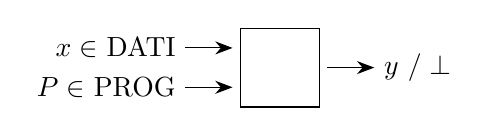
\begin{tikzpicture}

    \draw[-{Stealth[length=2.2mm]}] (2.3,1.75) node[left]{$x\in$\ DATI} -- (2.9,1.75);
    \draw[-{Stealth[length=2.2mm]}] (2.3,1.25) node[left]{$P\in$\ PROG} -- (2.9,1.25);
    \draw (3,2) rectangle (4,1);
    \node at (3.45,1.5) {$\C$};
    \draw[-{Stealth[length=2.2mm]}] (4.1,1.5) -- (4.7,1.5)
        node [right] {$y\ /\perp$};

\end{tikzpicture}
\end{figure}

La figura mostra il sistema di calcolo $\C$ che, preso un programma $P$
su input $x$, restituisce in output il risultato $y$ o il valore $\perp$
se il programma va in loop.

DATI è l'insieme di tutti i possibili dati di input e PROG l'insieme di
tutti i possibili programmi.

Il sistema di calcolo $\C$ non fa altro che eseguire il programma $P$ su input
$x$ ricavandone il risultato $y$:
\begin{equation}\label{eq:sistema_calcolo}
\C:\text{PROG}\times\text{DATI}\rightarrow\text{DATI}_\perp
\end{equation}

Quello che fa il programma $P$ è trasformare il dato di input $x$ in un dato
di output $y$; si può quindi dire che un programma non è altro che
una funzione che agisce da DATI in DATI:
$$ P:\text{DATI} \rightarrow \text{DATI}_\perp $$
$$ \Downarrow $$
\begin{equation}\label{eq:prog_dati} \text{PROG} =
\text{DATI}^{\text{DATI}}_\perp \end{equation}

La funzione associata al programma $P$ è detta \textbf{semantica di $P$}.

Da (\ref{eq:sistema_calcolo}) e (\ref{eq:prog_dati}) si ottiene che:
$$ \C:\text{DATI}^{\text{DATI}}_\perp\times\text{DATI}
\rightarrow\text{DATI}_\perp $$

$\C$ è una funzione di valutazione; $\C(P,x)$ è infatti la semantica di $P$.

\subsection{Potenza computazionale di \texorpdfstring{$\C$}{C}
\label{sec:pot_comp}}
Si definisce potenza computazionale di $\C$:
$$ F(\C) = \{\C(P,\_):P\in\text{PROG}\} \subseteq \text{DATI}^{\text{DATI}}_\perp $$
\textbf{$F(\C)$ contiene tutto ciò che un qualsiasi sistema di calcolo $\C$
può calcolare}. Quindi, per stabilire cosa l'informatica può risolvere, basta stabilire
il carattere dell'inclusione:
\begin{itemize}
    \item $F(\C)\subset\text{DATI}^{\text{DATI}}_\perp \Rightarrow $
        esistono problemi che l'informatica non può risolvere;
    \item $F(\C)=\text{DATI}^{\text{DATI}}_\perp \Rightarrow $
        l'informatica può risolvere tutto.
\end{itemize}

\subsection{Cardinalità di insiemi infiniti}
Per riuscire a capire se l'inclusione
$F(\C)\subseteq\text{DATI}^{\text{DATI}}_\perp$ sia propria o meno, si confronterà
la cardinalità dei due insiemi. Infatti dalla cardinalità si può ricavare che:
\begin{itemize}
    \item Se $|F(\C)|<\left|\text{DATI}^{\text{DATI}}_\perp\right|
    \quad \Rightarrow \quad F(\C)\subset\text{DATI}^{\text{DATI}}_\perp$;
    \item Se $|F(\C)|=\left|\text{DATI}^{\text{DATI}}_\perp\right|
    \quad \Rightarrow \quad F(\C)=\text{DATI}^{\text{DATI}}_\perp$.
\end{itemize}

Il concetto di cardinalità è semplice quando si tratta di insiemi finiti: basta
contare il numero di elementi che compongono l'insieme. Tuttavia, in presenza
di insiemi infiniti le cose si complicano.

Per esempio, si confrontino $\N$ e $\RN$: entrambi hanno cardinalità infinita
($|\N|=|\RN|=\infty$) eppure $\N\subset\RN$! Per comprendere quindi meglio
la cardinalità di insiemi infiniti si dovrà andare più nel dettaglio.

\subsubsection{Relazione binaria}
Si definisce relazione binaria $R$ sull'insieme $A$, un elenco di coppie ordinate
di elementi di $A$: $R\subseteq A^2$. Due elementi $a,b\in A$ sono in relazione 
$R$ se $(a,b)\in R$. Si usa la notazione:
\begin{itemize}
    \item $a \ R \ b$: $a$ è in relazione $R$ con $b$;
    \item $a\ \cancel{R} \ b$: $a$ non è in relazione $R$ con $b$;
\end{itemize}

\subsubsection{Relazione di equivalenza}
$R\subseteq A^2$ è una relazione di equivalenza se gode di:
\begin{enumerate}
    \item Riflessività: $\forall a \in A \quad a \ R \ a$
    \item Simmetria: $\forall a,b \in A \quad a \ R \ b \ \Leftrightarrow \ b \ R \ a$
    \item Transitività: $\forall a,b,c \in A \quad a \ R \ b
    \ \wedge \ b \ R \ c \Rightarrow a \ R \ c $
\end{enumerate}

\subsubsection{Classe di equivalenza}
Si definisce classe di equivalenza $[a]_R$ l'insieme degli elementi in relazione $R$
con $a$:
$$ [a]_R =\{b\in A: a \ R \ b\} $$

Tutte le classi di equivalenza di $R$ formano una partizione di $A$. L'insieme $A$
partizionato attraverso le classi di equivalenza di $R$ è detto \textbf{quoziente}
di $A$ rispetto a $R$ ed è denotato da $\sfrac{A}{R}$.

\subsubsection*{Esempio}
Si consideri la relazione $\equiv_4\subseteq\N^2$ di equivalenza modulo 4. Due numeri
sono in relazione di equivalenza modulo 4 se il resto della divisione per 4 è uguale
per entrambi.
$$ 5\equiv_4 9\ , \ 10\equiv_4 2 \ , \ \dots $$

Le classi di equivalenza sono:
\begin{align}
    [0]_4&=\{4k\}\tag{Multipli di 4}\\
    [1]_4&=\{4k+1\}\tag{Resto 1}\\
    [2]_4&=\{4k+2\}\tag{Resto 2}\\
    [3]_4&=\{4k+3\}\tag{Resto 3}
\end{align}
L'insieme $\{[0]_4,[1]_4,[2]_4,[3]_4\}=\sfrac{\N}{\equiv_4}$ è una partizione di $\N$.

\subsubsection{Insiemi isomorfi}
Due insiemi $A$ e $B$ sono \textbf{isomorfi} (o equinumerosi) se esiste una funzione
biettiva tra essi. Formalmente si indica con:
$$ A\sim B $$
La relazione di isomorfismo $\sim$ è una relazione di equivalenza in quanto:
\begin{enumerate}
    \item Riflessiva: si usi la funzione identità;
    \item Simmetrica: se esiste una funzione biettiva allora anche la sua inversa
        è biettiva;
    \item Transitiva: la composizione di due funzioni biettive è una funzione biettiva.
\end{enumerate}

Sia $\mathcal{U}$ l'insieme universo, ovvero l'insieme che contiene tutti gli insiemi.
Il quoziente di $\mathcal{U}$ rispetto a $\sim$ ($\sfrac{\mathcal{U}}{\sim}$) definisce il 
concetto di cardinalità:

\begin{figure}[H]
    \centering
    \begin{tikzpicture}[scale=1.5]

    \node at (-2,1) {$\sfrac{\mathscr{U}}{\sim}$};

    \draw[thick] (0,0) node{...} ellipse (2 and 1);
    \draw (-1.25,-.78) -- (-1.25,.78);
    \draw (-.5,-.97) -- (-.5,.97);
    \draw (.5,-.97) -- (.5,.97);
    \draw (1.25,-.78) -- (1.25,.78);

    \draw[fill,blue] (-.875,0) circle (.02);
    \draw[->,blue] (-.875,0) -- (-1.75,-1);
    \node[blue,below] at (-1.75,-1) {Classe di equivalenza};

\end{tikzpicture}
\end{figure}

Ogni partizione di $\sfrac{\mathcal{U}}{\sim}$ contiene gli insiemi tra loro isomorfi, ovvero
che hanno la stessa cardinalità.

\subsubsection*{Insiemi finiti}
Si definisca la famiglia di insiemi: 
$$J_n=\begin{cases}
\cancel{O} & n=0\\
\{1,\dots ,n\} & n>0
\end{cases}$$
$$ J_0=\{\}\ , \ J_1=\{1\} \ , \ J_{2}=\{1,2\} \ , \ J_{3}=\{1,2,3\}\ , \ \dots $$

Un'insieme $A$ ha cardinalità finita se $\exists n\in\N : A\sim J_n$ e si può dire che
$|A|=n$.

\subsubsection*{Insiemi infiniti}
Un insieme che non è finito ha cardinalità infinita.

\subsubsection{Insiemi numerabili}
Un insieme $A$ è numerabile se $\N\sim A$ (ovvero $A\in [\N]_\sim$). Vuole quindi dire
che esiste una biezione $f:\N\rightarrow A$ che permette di listare $A$ come:
$$ A = \{f(0),f(1),f(2),\dots\} $$
senza tralasciare nessun elemento.
\subsubsection*{Esempi}
\begin{tabular}{r l}
    PARI :& $f(n)=2n$ \\
    DISPARI :& $f(n)=2n+1$ \\
    $\mathbb{Z}$ :& mappo i pari nei non-negativi e i dispari nei negativi \\
    $\{0\}\cup 1\{0,1\}^*$ :& converto da binario a decimale \\
\end{tabular}

\subsubsection{Insiemi non numerabili}
Gli insiemi non numerabili sono insiemi a cardinalità infinita ma non listabili come
$\N$ (sono \quotes{più fitti}). Il re di questi insiemi è $\RN$.

\begin{theorem}
    $\RN$ è un insieme non numerabile: $$ \N \nsim \RN $$
\end{theorem}
\begin{proof} Per dimostrarlo dimostro che:
    \begin{enumerate}
        \item $\RN \sim (0,1)$: la biezione è rappresentata graficamente in figura:
            \vspace{-.2cm}
            \begin{figure}[H]
                \centering
                \begin{tikzpicture}[scale=2]

    \draw (-1.7,0) -- (1.7,0);
    \draw[densely dashed] (-1.7,0) -- (-2,0);
    \draw[densely dashed] (1.7,0) -- (2,0);
    \draw (0,.05) -- (0,-.05) node[below] {0};
    
    \draw[cyan] (1,1.5) arc[start angle=0, end angle=-180,radius=1];

    \draw (-1,1.5) -- (1,1.5);
    \draw (-1,1.55) -- (-1,1.45) node[left] {0};
    \draw (1,1.55) -- (1,1.45) node[right] {1};

    \draw[densely dashed, cyan] (-.515,.64) --  (0,1.5);
    \draw[red] (-.9,0) -- (-.515,.64) -- (-.515,1.5);
    \draw (-.515,1.45) -- (-.515,1.55) node[above] {$f(a)$};
    \draw (-.9,.05) -- (-.9,-.05) node[below] {$a$};

    \draw[densely dashed, cyan] (.68,.77) -- (0,1.5);
    \draw[red] (1.4,0) -- (.68,.77) -- (.68,1.5);
    \draw (.68,1.45) -- (.68,1.55) node[above] {$f(b)$};
    \draw (1.4,.05) -- (1.4,-.05) node[below] {$b$};

    \draw [fill] (0,1.5) circle (.02);

\end{tikzpicture}
            \end{figure}\vspace{-.6cm}
            (In realtà $\RN$ è isomorfo a un suo qualsiasi intervallo).
        \item $\N \nsim (0,1)$: dimostrazione per assurdo: assumo che $\N \sim (0,1)$;
            Questo vorrebbe dire che tutti i numeri compresi tra 0 e 1 sono numerabili.
            Elenco tutti i numeri associandoli a un numero naturale:

            \begin{minipage}{.45\textwidth}
                $$0\ \mapsto \ 0.{\color{red}a_{00}}\ a_{01}\ a_{02}\ a_{03}\ a_{04}\ \dots$$
                $$1\ \mapsto \ 0.a_{10}\ {\color{red}a_{11}}\ a_{12}\ a_{13}\ a_{14}\ \dots$$
                $$2\ \mapsto \ 0.a_{20}\ a_{21}\ {\color{red}a_{22}}\ a_{23}\ a_{24}\ \dots$$
                $$3\ \mapsto \ 0.a_{30}\ a_{31}\ a_{32}\ {\color{red}a_{33}}\ a_{34}\ \dots$$
                $$4\ \mapsto \ 0.a_{40}\ a_{41}\ a_{42}\ a_{43}\ {\color{red}a_{44}}\ \dots$$
                $$\vdots\qquad\vdots\qquad\vdots\qquad\vdots\qquad\vdots\qquad\ddots$$
                \vspace{.4cm}
            \end{minipage}
            \begin{minipage}{.48\textwidth}
                $a_{ij}$ è la $i$-esima cifra dopo lo zero del $j$-esimo numero
                nella lista.

                Se $(0,1)$ fosse numerabile tutti i suoi numeri dovrebbero far parte
                della lista.

                Si consideri il numero:
                $$ 0.c_0c_1c_2c_3\dots $$

                con: $$ c_i = \begin{cases}
                2 & a_{ii}\neq2\\
                3 & a_{ii}=2
                \end{cases} $$

            \end{minipage}
            Chiaramente $0.c_0c_1c_2c_3\dots\in(0,1)$ ma non appare nella lista:
            \begin{itemize}
                \item Differisce dal primo numero perchè $c_0\neq a_{00}$;
                \item Differisce dal secondo numero perchè $c_1\neq a_{11}$;
                \item $\dots$
                \item Differisce da qualunque numero nella lista sulla cifra 
                    {\color{red} diagonale}.
            \end{itemize}
            Ho trovato l'assurdo quindi $\N \nsim (0,1)$ (dimostrazione per 
            diagonalizzazione).
    \end{enumerate}
    Sfruttando la transitività di $\sim$ posso si può affermare quindi che:
    $$ \RN \underset{(1)}{\sim} (0,1) \underset{(2)}{\nsim} \N \quad \Rightarrow \quad \RN \nsim \N $$
\end{proof}

Tutti gli insiemi isomorfi a $\RN$ sono detti continui. Altri insiemi non numerabili sono:
\begin{itemize}
    \item Insieme delle parti di $\N$: $2^\N = \{\text{sottoinsiemi di } \N\}$
    \item Insieme delle funzioni da $\N$ a $\N$:
        $\N^\N_\perp = \{f:\N\rightarrow\N_\perp\}$
\end{itemize}

\subsection{Esistono funzioni non calcolabili?}
Ora che il concetto di cardinalità è più chiaro, si riprenda il concetto di 
potenza computazionale di un sistema di calcolo $\C$ (paragrafo \ref{sec:pot_comp}):
$$
F(\C) = \{\C(P,\_):P\in\text{PROG}\} \subseteq \text{DATI}^{\text{DATI}}_\perp
$$

Per definizione $F(\C)$ ha la stessa numerosità di PROG:
$$ F(\C) \sim \text{PROG} $$

Ragionevolmente, \textbf{ma non formalmente}, si può notare che:
\begin{itemize}
    \item PROG$\sim\N$: si prenda la stringa binaria con la quale il programma è
        salvato sul disco e si converta da binario a decimale;
    \item DATI$\sim\N$: si applichi lo stesso ragionamento del punto precedente.
\end{itemize}
Ne segue che:
$$ F(\C) \sim \text{PROG} \sim \N \nsim\N^\N_\perp\sim \text{DATI}^\text{DATI}_\perp$$
$$ \Downarrow $$
$$ F(\C) \nsim \text{DATI}^\text{DATI}_\perp $$
$$ \Downarrow $$
$$ F(\C) \subset \text{DATI}^\text{DATI}_\perp $$

Quello che questa osservazione dice è che ho pochi programmi ($\N$) e troppe
funzioni ($\N^\N_\perp$).
\textbf{Alla domanda \quotes{Esistono funzioni non calcolabili?} si può quindi 
rispondere con un sì!}

\subsubsection{DATI numerabile}
Obiettivo di questa sezione è dimostrare formalmente che:
$$ \text{DATI} \sim \N $$
Vogliamo quindi trovare una biezione che è in grado di associare biunivocamente
dei dati a un numero e quindi anche di ottenere i dati di partenza dal
numero. Per farlo si userà il seguente teorema.

\begin{theorem}
    $\N\times\N\sim\N^+$
\end{theorem}
\begin{proof}
    Si definisca la funzione coppia di Cantor $\cantor{\ ,\ }$:
    $$ \cantor{\ ,\ }:\N\times\N\rightarrow\N^+ $$
    $\cantor{\ ,\ }$ associa biunivocamente una coppia di numeri $x$ e 
    $y$ a un numero $n$:
    $$ \cantor{x,y} = n $$
    La mappa che $\cantor{\ ,\ }$ usa per assegnare i valori di ogni coppia viene 
    descritta nelle seguenti tabelle:

    \begin{minipage}{.48\textwidth}
        \centering
        \begin{tabular}{c|c c c c c c}
            $x\backslash y$&0 &1 &2 &3 &4\\ \hline
               0 &1 &3 &6 &10&15\\
               1 &2 &5 &9 &14&...\\
               2 &4 &8 &13&...&  \\
               3 &7 &12&...&  &  \\
               4 &11&...&  &  &  \\
               5 &$\nearrow$&&&&\\
        \end{tabular}
    \end{minipage}
    \begin{minipage}{.48\textwidth}
        \centering
        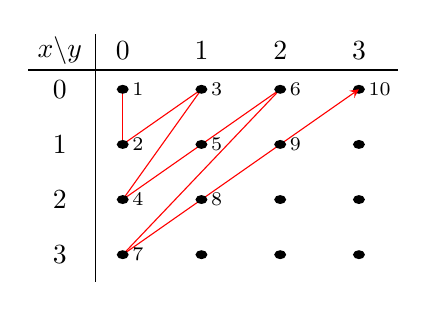
\begin{tikzpicture}[yscale=.7]
    \usetikzlibrary{arrows.meta}

    \tikzset{
        myarrow/.style=-stealth
    }

    \foreach \x in {0,1,2,3} {
        \node at (.2,-\x-1) {\x};
    }
    \foreach \y in {0,1,2,3} {
        \node at (\y+1,-.3) {\y};
    }
    \draw[red] (1,-1) -- (1,-2);
    \draw[red] (1,-2) -- (2,-1);
    \draw[red] (2,-1) -- (1,-3);
    \draw[red] (1,-3) -- (3,-1);
    \draw[red] (3,-1) -- (1,-4);
    \draw[red] (1,-4) -- (3+.2,-2+.2);

    \node at (.2,-.3) {$x\backslash y$};
    \foreach \x in {0,1,2,3} {
        \foreach \y in {0,1,2,3} {
            \ifthenelse{\x<\y \OR \x=\y}{
                \draw[thick,fill] (4-\y,-\x-1) circle (.06);
            }{}
        }
    }
    \draw[myarrow,red] (3+.2,-2+.2) -- (4,-1);
    \node[right] at (1,-1) {\scriptsize 1};
    \node[right] at (1,-2) {\scriptsize 2};
    \node[right] at (2,-1) {\scriptsize 3};
    \node[right] at (1,-3) {\scriptsize 4};
    \node[right] at (2,-2) {\scriptsize 5};
    \node[right] at (3,-1) {\scriptsize 6};
    \node[right] at (1,-4) {\scriptsize 7};
    \node[right] at (2,-3) {\scriptsize 8};
    \node[right] at (3,-2) {\scriptsize 9};
    \node[right] at (4,-1) {\scriptsize 10};

    \draw (-.2,-.65) -- (4.5,-.65);
    \draw (.65,0) -- (.65,-4.5);

\end{tikzpicture}
    \end{minipage}

    Si vuole calcolare ora la forma analitica di $\cantor{\ ,\ }$; si prenda una generica
    coppia di numeri $\cantor{x,y}$:

    \begin{minipage}{.4\textwidth}
        \centering
        \begin{tikzpicture}[yscale=.8]
    \usetikzlibrary{arrows.meta}

    \newcommand{\smallerplus}{\raisebox{.3\height}{\scalebox{.6}{+}}}

    \draw[red,densely dashed] (1,-4) -- (3,-2);
    \draw[densely dashed] (.65,-2) -- (3,-2);
    \draw[densely dashed] (3,-1+.2) -- (3,-2);

    \node at (.1,-.3) {$x\backslash y$};

    \node at (2+1,-.3) {$y$};
    \node at (.9,-.3) {0};
    \node at (1+1,-.3) {$\dots$};
    \node at (.1,-1) {$\vdots$};
    \node at (.1,-1-1) {$x$};
    \node at (.1,-2-1) {$\vdots$};
    \node at (.05,-3-1-.05) {$x{\color{red}\smallerplus y}$};
    \def \offset {.28}
    \draw[white,fill] (3-\offset-.15,-2-\offset) rectangle (3+\offset+.05,-2+\offset-.05);
    \node at (3,-2) {$\cantor{x,y}$};
    \draw[white,fill] (1-\offset-.15,-4-\offset) rectangle (1+\offset+.05,-4+\offset-.05);
    \node[blue] at (1.1,-4) {$\cantor{x\smallerplus y,0}$};

    \draw (-.2,-.65) -- (4.5,-.65);
    \draw (.45,0) -- (.45,-4.5);

\end{tikzpicture}
    \end{minipage}
    \begin{minipage}{.58\textwidth}
        Per come è definita $\cantor{x,y}$ (vedi tabella precedente) si ha che:
        \begin{equation}\label{eq:cantor_analytic}
            \cantor{x,y} = {\color{blue}\cantor{x+y,0}}{\color{red}+y}
        \end{equation}

        Ora l'incognita da calcolare resta $\color{blue}\cantor{z,0}$ che,
        si può ottenere come:
        \begin{equation}\label{eq:cantor_analytic_2}
            \cantor{z,0} = \sum_{i=0}^z i+1 = \frac{z(z+1)}{2}+1
        \end{equation}
    \end{minipage}
    
    Da (\ref{eq:cantor_analytic}) e (\ref{eq:cantor_analytic_2}) segue che:
    $$ \cantor{x,y} = \cantor{x+y,0}+y = \frac{(x+y)(x+y+1)}{2}+y+1 $$
    
    $\cantor{\ ,\ }$ si dimostra quindi mappare univocamente le coppie di numeri
    in numeri ($\N^2\rightarrow\N^+$). Si cercherà ora di mostrare il passaggio inverso, 
    ovvero come riottenere la coppia di numeri dal numero risultante
    ($\N^+\rightarrow\N^2$).

    Si definiscano le seguenti funzioni:
    $$ \cantor{x,y} = n \quad , \quad sin(n) = x \quad , \quad des(n) = y $$

    Da (\ref{eq:cantor_analytic}) si ha che:
    $$ \begin{aligned}
        y &= \cantor{x,y}-\cantor{x+y,0} \\
          &= n-\cantor{x+y,0} \\
          &= n-\cantor{\gamma,0} \\
    \end{aligned} $$
    Il valore di $\gamma$ è il più grande valore che, messo sulla prima colonna
    ($\cantor{\gamma,0}$) non supera $n$:
    $$ \gamma = \max\{z\in\N:\cantor{z,0}\leq n\} $$
    $$ \cantor{z,0}\leq n $$
    $$ \frac{z(z+1)}{2}+1 \leq n $$
    $$ z^2+z+2-2n\leq 0 $$
    $$ \frac{-1-\sqrt{8n-7}}{2}\leq z \leq \frac{-1+\sqrt{8n-7}}{2} $$
    $$ \Downarrow $$
    $$ \gamma=\left\lfloor\frac{-1+\sqrt{8n-7}}{2}\right\rfloor $$
    
    In conclusione:
    $$ des(x) = n-\cantor{\gamma,0} $$
    $$ sin(x) = \gamma-des(x) $$

    La funzione coppia di Cantor $\cantor{\ ,\ }$ si è quindi mostrata
    essere una biezione tra $\N^+$ e $\N^2$ mostrando che i due insiemi
    hanno la stessa cardinalità.
\end{proof}

È facile poi, partendo da $\cantor{\ ,\ }$, creare una biezione tra $\N$ e $\N^2$
(dimostrando che $\N\times\N\sim\N$):
$$ [\ ,\ ]:\N\times\N\rightarrow\N $$
$$ [x,y] = \cantor{x,y}-1 $$

Il precedente risultato mette alla luce anche che:
$$ \mathbb{Q}\sim\N $$
in quanto ogni suo elemento non è altro che una coppia di numeri messi
a frazione.